\documentclass{article}

\usepackage[utf8]{inputenc}
\usepackage[ngerman]{babel}
\usepackage[T1]{fontenc}
\usepackage{enumitem}
\usepackage{graphicx}
\usepackage{float}

\newlist{FA}{enumerate}{1}
\setlist[FA]{label=/FA\arabic*/}

\newlist{NA}{enumerate}{1}
\setlist[NA]{label=/NA\arabic*/}

\newlist{PD}{enumerate}{1}
\setlist[PD]{label=/PD\arabic*/}

\title{\textbf{Pflichtenheft} \\ Cryptographics}
\author{}
\date{\today}

\usepackage[ngerman]{translator}
%Paket laden
\usepackage{hyperref}
\usepackage[nonumberlist, section=subsection]{glossaries}
 
 
%Glossar-Befehle anschalten
\makeglossaries

\newglossaryentry{Cryptographics}{name={Cryptographics}, description={Name des zu entwickelnden Produkts}}
\newglossaryentry{Kryptologikum}{name={Kryptologikum}, description={Ausstellung des IKS}}
\newglossaryentry{PSE}{name={PSE}, description={Praxis der Software-Entwicklung}}
\newglossaryentry{IKS}{name={IKS}, description={Institut für Kryptographie und Sicherheit}}
\newglossaryentry{KIT}{name={KIT}, description={Karlsruher Institut für Technologie}}


\begin{document}

% The cover page.
\maketitle
\begin{table}[b]
  \begin{tabular}{| l | l | l |}
    \hline
    \textbf{Phase} & \textbf{Verantwortlicher} & \textbf{Email} \\ \hline
    Pflichtenheft & Matthias Jaenicke & matthias.jaenicke@student.kit.edu \\ \hline
    Entwurf & Matthias Plappert & undkc@student.kit.edu \\
            & Julien Duman & uncyc@student.kit.edu \\ \hline
    Implementierung & Christian Dreher & uaeef@student.kit.edu \\ \hline
    Qualitätssicherung & Wasilij Beskorovajnov & uajkm@student.kit.edu \\ \hline
    Präsentation & Aydin Tekin & aydin.tekin@student.kit.edu \\ \hline
    \end{tabular}
\end{table}
\newpage

% Table of contents page.

\tableofcontents
\newpage

% Start of the actual document.
\section{Zielbestimmung}

Im Rahmen der \gls{PSE}-Veranstaltung soll für das \gls{Kryptologikum} des Instituts für
Kryptographie und Sicherheit die Software \gls{Cryptographics} zur
Demonstration kryptographischer Verfahren erstellt werden. \\
\\
Das Programm soll im Laufe der Ausstellung \gls{Kryptologikum} das Interesse der Besucher wecken, sich mit Verschlüsselung zu befassen und schließlich auch ausgewählte Inhalte der Kryptographie näher bringen. \\
\\
Wichtig ist, dass die Visualisierungen ansprechend und verständlich gestaltet sind. Die Nutzung von \gls{Cryptographics} soll Spaß machen. \\
\\
Jedes Verfahren wird in drei Schritten vorgestellt. Diese sind eine automatisch ablaufende Demonstration, ein interaktiver Versuch und ein Wiki-artiger Artikel für weitere Informationen.
In der Demonstration wird dem Nutzer der Ablauf der Verschlüsselung möglichst anschaulich demonstriert. Darauf folgend kann im Eigenversuch auf der gleichen Oberfläche die Verschlüsselung selbst ausprobiert werden. Dem Nutzer wird hierbei eine größtmögliche Freiheit zur Wahl sämtlicher Komponenten (wie Klartext, Primzahl, etc.) gelassen. Unter ``Mehr Wissen'' sollen sich interessierte Benutzer schließlich tiefgehender über das Verfahren informieren können, über seine Entstehung, Einsatz und Nachfolger. Auf geeignete weiterführende Literatur kann mit QR-Codes verwiesen werden. \\

\subsection{Musskriterien}

\begin{itemize}
    \item Visualisierung Caesar-Chiffre
    \item Visualisierung Vigenère-Chiffre
    \item Visualisierung Diffie-Hellmann
    \item Zugriff auf Krypto-Verfahren über Zeitleiste
    \item Benutzerführung über Phasen
    \item Krypto-Algorithmen lassen sich schrittweise ausführen, um den Prozess
        langsam zu verdeutlichen
    \item Angeleiter Selbstversuch bei komplexen Verfahren
    \item Praxisbezug auf moderne Kryptoverfahren
    \item Time-Out bei fehlender Nutzerinteraktion, Rückkehr zum Startbildschirm
    \item Mögliche Rückkehr zur Startoberfläche per Button zu jedem Ausführungszeitpunkt
    \item Interaktion des Benutzers über den Touchscreen
    \item Intuitive Benutzerführung
    \item Einfache, übersichtliche UI, die sich gut auf Touchscreen bedienen lässt
    \item Einheitliche optische Darstellung der verschiedenen Verfahren
    \item Robuste Programmierung
    \item Schnelle Reaktionszeiten
    \item Robustheit gegen au"sergewöhnliche Interaktion
    \item Beenden des Programms / Wechsel zum Desktop nur per angeschlossener Tastatur, nicht über Touch-Eingabe
    \item Vermeidung undefinierter Zustände des Programms
    \item Vermeidung von Sackgassen im Programm, die einen Neustart erfordern
    \item Lauffähigkeit des Programms in jedem vollständigen Java RTE
\end{itemize}

\subsection{Wunschkriterien}

\begin{itemize}
    \item Visualisierung Public Key – Infrastruktur
    \item Visualisierung Shamir Secret Sharing
    \item Visualisierung Passwortsicherheit
    \item Visualisierung One-Time-Pad
    \item Visualisierung Blockchiffre (DES, AES)
    \item Visualisierung Hashfunktionen
    \item Visualisierung RSA
    \item Modulares Austauschen / Hinzufügen von weiteren kryptografischen Verfahren
    \item Animation auf Startbildschirm als Blickfang
    \item Namen / Icons für Verfahren in der Zeitleiste für bessere Übersichtlichkeit
    \item Literaturhinweise (auch weiterführende Literatur) mittels QR-Codes
    \item Optisch ansprechende Visualisierungen durch Nutzung von Grafiken und Animationen
    \item Verbesserte Verständlichkeit der Visualisierungen durch Verwendung von z.B. Analogien
    \item Visualisierung von Angriffen auf Verfahren
    \item Erfassung von grundlegenden Nutzungsstatistiken zur potentiellen externen Analyse des Nutzerverhaltens  im Hinblick auf eventuelle zukünftige Optimierung des Programms
\end{itemize}

\subsection{Abgrenzungskriterien}
\begin{itemize}
	\item Implementierung sämtlicher kryptologischer Verfahren nur zu Vorführungszwecken; somit keine festgelegt sichere Implementierung
    \item Keine optimierte und 100\% standardkonforme Implementierung von Krypto-Algorithmen,
        sondern Fokus auf schrittweiser Ausführbarkeit
    \item Keine formale Korrektheit bei Erklärungen sondern Ansatz ohne nötige Vorkenntnisse
        um breiter Masse zugänglich zu sein
    \item Nicht zur tatsächlichen Verschlüsselung von Texten gedacht
\end{itemize}

\section{Produkteinsatz}
\subsection{Anwendungsbereiche}
\gls{Cryptographics} soll in erster Linie als Ausstellungsstück für das \gls{Kryptologikum} des Instituts für Kryptographie und Sicherheit (\gls{IKS}) am Karlsruher Institut für Technologie (\gls{KIT}) dienen.

Besuchern der Ausstellung soll das Funktionsprinzip und die Verwendung historischer, sowie aktueller, kryptographischer Verfahren nähergebracht werden. Diese sollen anhand von vereinfachten und beispielhaften Szenarien aus dem Alltag vermittelt werden, mit dem Ziel, ein größeres Interesse an der Materie zu wecken.

\gls{Cryptographics} soll primär auf dem eeePC (siehe Produktumgebung) im \gls{Kryptologikum} eingesetzt werden.

\subsection{Zielgruppen}

Das Programm richtet sich insbesondere an Kinder, Jugendliche und Erwachsene mit grundlegenden Kenntnissen der Mathematik. Die Zielgruppe ist demnach ein anonymes Publikum, das sich potenziell aus fachfremden Personen zusammensetzt. Deshalb dürfen für die Verwendung von \gls{Cryptographics} keine Vorkenntnisse in der Kryptographie vorausgesetzt werden.

\subsection{Betriebsbedingungen}

\gls{Cryptographics} soll im Dauerbetrieb problemlos laufen. Dementsprechend dürfen keine Ausnahmen auftreten, die den Betrieb des Programms behindern, oder gar einen Absturz auslösen, der den Benutzer zur Betriebssystemebene führt. Insbesondere muss darauf geachtet werden, dass schnelle, unkontrollierte Benutzereingaben zu keinem undefinierten Zustand des Programms führen. Auch ein reguläres Beenden von \gls{Cryptographics} soll durch den Benutzer nicht möglich sein, und nur durch eine angeschlossene Hardwaretastatur erreicht werden können.

Der Betrieb soll für die Hardware des eeePC (siehe Produktumgebung) optimiert sein, der während der Ausstellung über keine Internetverbindung verfügt. Inhalte zu weiterführenden Informationen müssen also lokal in Form von leicht aktualisierbaren und austauschbaren Textdateien vorliegen.

\section{Produktumgebung}

\gls{Cryptographics} wird nicht ausschließlich, aber primär für folgende Spezifikationen entwickelt.

\subsection{Software}

\begin{itemize}
	\item Windows XP Home edition
	\item Java Version 7 Update 45
\end{itemize}

\subsection{Hardware}

\begin{itemize}
	\item ASUS Touchscreen EeeTop Tablet
	\item 1.6 GHz Intel Atom CPU
	\item 1GB RAM
	\item 160GB HDD
	\item 15.6 Zoll LCD (1366x768 Px Auflösung)
	\item Integrierter Grafikchip
	\item Resistiver Touchscreen
\end{itemize}

\section{Produktfunktionen}

\subsection{Funktionale Anforderungen}

\subsubsection{Grundfunktionen}

\begin{FA}[start=100]
  \item Darstellung eines Startbildschirm mit Zeitleiste
  \item Darstellung aller Visualisierungen auf einer Zeitleiste
  \item Interaktion mit der Zeitleiste, um eine einzelne Visualisierung auswählen zu können
  \item Darstellung einer Übersichtsseite zur gewählten Visualisierung
  \item Start der gewählten Visualisierung
  \item Abbruch einer gewählten Visualisierung, um zum Startbildschirm zurückzukehren
  \item Soforthilfe zu einer gewählten Visualisierung
  \item Darstellung weiterführender Information nach erfolgreichem Beenden einer Visualisierung 
\end{FA}

\begin{FA}[start=100]
 \item Prozess: Visualiserung des Verfahrens Cäsar.
\end{FA}
\begin{itemize}[label={}]
 \item Ziel: Benutzer versteht das Verfahren und kann selbstständig 
 beliebigen Klartext verschlüsseln und beliebigen Chiffrat, der mit Cäsar erzeugt wurde, entschlüsseln.
 \item Aktuere: Benutzer.
 \item Beschreibung:
 \item Phase1: Demonstration.
\begin{enumerate}[]
 \item Auf dem Bildschirm erscheinen Animationen, die das Verfahren erklären.
 \item Der Benutzer sieht die Animation schrittweise und kann sie jederzeit anhalten.
 \item Der Benutzer kann in der Animation einen Schritt vorwärts gehen.
 \item Der Benutzer kann in der Animation einen Schritt rückwärts gehen. 
 \item Am Ende der Demonstration wechselt die Visualisierung des Verfahrens in die zweite Phase, dem Selbstversuch.
\end{enumerate}
 \item Phase2: Selbstversuch.
 \item Schritt 1:
 \begin{enumerate}
  \item Der Benutzer wird mit einem kleinen Eingabefenster aufgefordert eine kurze Eingabe, 
        die aus einer kleinen Zeichenfolge besteht, zu tätigen.
  \item Benutzer hat die Möglichkeit sich die Eingabe durch einen Button generieren zu lassen.
  \item Eingabe ist nun in der Mitte des Bildschirms zu sehen und unterhalb ist das Alphabet 
        abgebildet, wobei jeder Buchstabe nummeriert ist.     
  \item Nun leuchtet jeder Buchstabe der Eingabe nacheinander auf.
  \item Der Benuter wählt das verschlüsselte Gegenstück zum leuchtenden Zeichen in der Eingabe aus dem Alphabet aus. 
  \item Bei jeder Auswahl des Buchstaben aus dem Alphabet taucht dieser unter der Eingabe auf.
  \item[] Benutzer wiederholt alles solange, bis alle Buchstaben der Eingabe abgearbeitet sind und 
        das Chiffrat vollständig unter der Eingabe dargestellt ist.
  \item Nun entschlüsselt das Programm das Chiffrat selbst.
  \item Programm zeigt die Ausgabe unterhalb des Chiffrats an.
 \end{enumerate}
 \item Schritt 2:
 \begin{enumerate}
  \item Die alte Bildschirmanzeige verschwindet.
  \item Für den Benuter wird vom Programm ein Chiffrat generiert. 
  \item[] Auf diesem Chiffrat wird dann analog gearbeitet, wie auf der Eingabe aus Schritt 1. Die Funktionalen 
          Anforderungen sind identisch. Die Unterschiede liegen darin, dass der Benutzer nun entschlüsselt.
  \item Nach erfolgreichem Entschlüsseln wechselt die Visualisierung des Verfahrens in die Phase 3, 
        Wiki.
 \end{enumerate}
 \item Phase 3: Wiki.
  \begin{enumerate}
   \item Sammlung an Artikeln über das Verfahren Cäsar.
   \item Nach dem Durchlesen ist die Visualisierung des Verfahrens Cäsar abgeschlossen. 
         Der Benuter wird zum nächsten Verfahren weitergeleitet.
  \end{enumerate}
\end{itemize}



%/Vigenere Visualiserung, Funktionale Anforderungen.
\begin{FA}[start=100]
 \item Prozess: Visualiserung des Verfahrens Vigenere.
\end{FA}
\begin{itemize}[label={}]
 \item Ziel: Benutzer versteht das Verfahren und kann selbstständig beliebigen Klartext verschlüsseln und beliebigen Chiffrat, 
       der mit Vigenere erzeugt wurde, entschlüsseln.
 \item Akteure: Benutzer.
 \item Beschreibung:
 \item Phase1: Demonstration.
 \item Identisch mit funktionalen Anforderungen in Caesar Phase 1, Demonstration. 
 \item Phase2: Selbstversuch.
 \item Schritt 1:
 \begin{enumerate}
  \item Auf dem Bildschirm erscheinen Animationen, die das Verfahren erklären.
  \item Der Benutzer kann die Animationen schrittweise vollziehen.
  \item Der Benutzer kann in den Animationen auch schrittweise rückwärts gehen. 
  \item Am Ende der Animation wechselt die Visualisierung des Verfahrens in die zweite Phase, dem Selbstversuch.
 \end{enumerate}
 \item Schritt 2:
 \begin{enumerate}
  \item Die alte Bildschirmanzeige verschwindet.
  \item Für den Benuter wird vom Programm ein Chiffrat mit einem Codewort generiert. 
  \item[] Auf diesem wird dann analog gearbeitet, wie auf der Eingabe aus Schritt 1. Die Funktionalen Anforderungen sind identisch.
        Die Unterschiede liegen darin, dass der Benutzer nun entschlüsselt. 
        Der Klartext in Schritt 1 ist nun das Chiffrat und der Schlüssel hat dieselbe Rolle.
        Das Chiffrat wird auf dieselbe Weise entschlüsselt, wie der Klartext verschlüsselt. 
  \item Programm prüft die entschlüsselte Zeichenfolge auf Richtigkeit.
  \item Nach erfolgreichem Entschlüsseln wechselt die Visualisierung des Verfahrens in die Phase 3, Wiki.
 \end{enumerate}
 \item Phase 3: Wiki.
 \item Identisch mit den funktionalen Anforderungen aus Cäsar, Phase 3: Wiki.
\end{itemize}
%/Ende der Funktionalen Anforderungen für die Visualiserung Vigenere's


\begin{FA}[start=100]
\item Prozess: Diffie-Hellman Schlüsselaustausch Demonstration
\end{FA}
\begin{itemize}[label={}]
    \item Ziel: Vermittlung des Diffie-Hellman Schlüsselaustauschs mit Farben-Analogie
    \item Vorbedingung: keine
    \item Nachbedingung (Erfolg): Alice und Bob haben sich auf eine
        gemeinsame, geheime Farbe geeinigt die Eve nicht kennt
    \item Nachbedingung (Fehlschlag): Gibt es nicht, da nur
        eine Demonstration ausgeführt wird
    \item Auslösendes Ereignis: Ausgewählt in der Zeitleiste
\end{itemize}

Beschreibung:
\begin{enumerate}
    \item Erkläre das Ziel sich auf ein gemeinsames Geheimnis zu einigen,
        durch Nutzung eines unsicheren Übertragungskanals
        bei dem Eve lauschen kann, ohne dass Eve das Geheimnis erfährt
    \item Demonstriere das Prinzip der Einwegfunktion, anhand Farben die man mischen
        kann. Farben zu mischen ist einfach, zur einer gemischten Farbe
        herauszufinden welche Farben verwendet wurden hingegen ist schwer
    \item Alice und Bob einigen sich auf eine gemeinsame, nicht geheime Farbe A
    \item Alice wählt eine geheime Farbe X und mischt sie mit A zur Farbe AX
    \item Bob wählt eine geheime Farbe Y und mischt sie mit A zur Farbe AY
    \item Alice schickt AX zu Bob u. Bob schickt AY zu Alice
    \item Alice mischt X mit AY zu AYX
    \item Bob mischt Y mit AX zu AXY
    \item Wenn Eve weder X noch Y erfahren hat, kennt Eve nicht AXY
\end{enumerate}

\begin{FA}[start=100]
\item Prozess: Diffie-Hellman Schlüsselaustausch Selbstversuch
\end{FA}
\begin{itemize}[label={}]
    \item Ziel: Der Nutzer hat einen erfolgreichen Diffie-Hellman Schlüsselaustausch
        (mit Farben-Analogie) mit Bob durchgeführt
    \item Vorbedingung: keine
    \item Nachbedingung (Erfolg): Alice und Bob haben sich auf eine
        gemeinsame, geheime Farbe geeinigt, die Eve nicht kennt
    \item Nachbedingung (Fehlschlag): Alice und Bob haben eine gemeinsame,
        nicht geheime Farbe oder sich auf gar keine Farbe geeinigt
    \item Auslösendes Ereignis: Ende der Demonstration des Diffie-Hellman
        Schlüsselaustauschs mit Farben, oder die Demonstration wurde Übersprungen
\end{itemize}

Beschreibung:
\begin{enumerate}
    \item Der Nutzer übernimmt die Rolle von Alice
    \item Benenne die Aufgabe, dass der Nutzer (Alice) sich auf ein gemeinsames Geheimnis
        mit Bob einigt, wobei ein öffentlicher Kanal genutzt wird auf dem Eve lauscht,
        ohne dass Eve das Geheimnis erfährt.
    \item Der Nutzer (Alice) wird aufgefordert eine Farbe A zu wählen,
        wurde diese gewählt, wird der Nutzer aufgefordert
        die nicht geheime Farbe an Bob zu schicken.
    \item Der Nutzer soll nun eine geheime Farbe X != A wählen,
        diese soll er an Bob schicken
    \item Bob wählt eine geheime Farbe Y und mischt sie mit A zur Farbe AY
    \item Der Nutzer kann nun eine Farbe zu Bob schicken,
        wenn er die private Farbe X schickt hat er verloren,
        wenn er A schickt hat er ebenso verloren,
        wenn er AX schickt geht es weiter
    \item Der Nutzer wird aufgefordert nun die richtigen Farben zu mischen,
        wenn er X mit AY mischt geht es weiter, wenn nicht hat er verloren.
    \item Bob mischt Y mit AX zu AXY
    \item Wenn Eve weder X noch Y erfahren hat, kennt Eve nicht AXY,
        der Nutzer kann beglückwünscht werden
\end{enumerate}

\subsubsection{Erweiterte Funktionen}


\begin{FA}[start=500]
\item Public Key Infrastruktur (PKI)
\end{FA}
\begin{itemize}[label={}]
\item Prozess: Erläuterung der Vorgänge bei der Verteilung von öffentlichen Schlüsseln.
\item Ziel: Dem Benutzer ist klar ersichtlich, wie die Verteilung vonstatten geht und welche Instanzen in diesem Rahmen 
            interagieren.
\item Akteure: Benutzer.
\item Beschreibung:
\item Phase 1:Demonstration.
\begin{enumerate}
 \item[1-4] Die ersten 4 funktionalen Anforderungen sind identisch mit den Anforderungen aus Cäsar und Vigenère. 
 \item[5] An die Demo anschließend springt das Programm in die Phase 3, Wiki. Phase 2 wird übersprungen, 
          da sich die Überlegungen zu einem Selbstversuch in PKI keine vernünftigen Ergebnisse liefern. 
          Ein Selbstversuch kann aber jederzeit eingebaut werden
\end{enumerate}
\item Phase 3: Wiki.
\begin{enumerate}
 \item[1-2] Identisch mit den funktionalen Anforderung aus Cäsar und Vigenère
\end{enumerate}.
\end{itemize}

\begin{FA}[start=600]
\item Hashing
\end{FA}
\begin{itemize}[label={}]
\item Prozess: Hashing Demonstration
\item Ziel: Dem Benutzer ist die Funktionsweise des Hashings bewusst und erhält einen Einblick in den praktischen Nutzen.
\item Akteure: Benutzer.
\item Beschreibung:
\item Phase 1: Einleitung.
\begin{enumerate}
\item Erkläre was Hashes sind.
\item Zeige deren praktischen Nutzen anhand von Beispielen in der Informationstechnologie.
\end{enumerate}
\item Phase 2: Animation.
\begin{enumerate}
\item Erkläre das Ziel "Fingerabdrücke" von Daten zu machen.
\item Demonstriere eine einfache Merkle-Damgard-Konstruktion.
\item Nehme einen festgelegten String und führe diese durch die Konstruktion.
\item Jeder Schritt wird einzeln visualisiert dargestellt, so entsteht Schritt für Schritt der "Fingerabdruck".
\item Gebe den Fingerabdruck dieses Strings an. Speichere das Ergebnis in der Maske, damit dieser später eingesehen werden kann.
\item Nun ersetze einen Buchstaben des vorherigen Strings und führe diese erneut durch die Konstruktion.
\item Nach dem Erhalten des zweiten Hashes, zeige Nutzer dass die Hashes sich gravierend unterscheiden, also dass Hashes ``echte Fingerabdrücke'' sind.
\end{enumerate}
\item Phase 3: Weiterführende Informationen.
\begin{enumerate}
\item Der Benutzer erhält Links zu weiterführenden Quellen.
\end{enumerate}
\end{itemize}

\begin{FA}[start=700]
\item Blockchiffren
\end{FA}
\begin{itemize}[label={}]
\item Prozess: Blockchiffren Demonstration
\item Ziel: Dem Benutzer ist die Funktionsweise von Blockchiffren bewusst und erhält einen Einblick in die verschiedenen Modí.
\item Akteure: Benutzer.
\item Beschreibung:
\item Phase 1: Einleitung.
\begin{enumerate}
\item Erkläre was Blockchiffren sind.
\item Zeige deren praktischen Nutzen anhand von Beispielen in der Informationstechnologie.
\end{enumerate}
\item Phase 2: Animation ECB.
\begin{enumerate}
\item Erkläre den ECB Modus.
\item Zeige den Aufbau vom ECB Modus.
\item Nehme einen festgelegten String und führe diese durch die Konstruktion.
\item Jeder Schritt wird einzeln visualisiert dargestellt, so entsteht Schritt für Schritt das Chiffrat.
\item Gebe das Chiffrat dieses Strings an. Speichere das Ergebnis in der Maske, damit dieser später eingesehen werden kann.
\item Nun ersetze einen Buchstaben des vorherigen Strings und führe diese erneut durch die Konstruktion.
\item Nach dem Erhalten des zweiten Chiffrates, zeige Nutzer dass der ECB Modus homomorph ist.
\item Zeige Nutzer das Problem das dadurch entsteht anhand einem im ECB Modus chiffrierten Bildes.
\item Dechiffriere das erste Chiffrat.
\end{enumerate}
\item Phase 3: Animation CBC.
\begin{enumerate}
\item Erkläre den CBC Modus.
\item Zeige den Aufbau vom CBC Modus.
\item Nehme einen festgelegten String und führe diese durch die Konstruktion.
\item Jeder Schritt wird einzeln visualisiert dargestellt, so entsteht Schritt für Schritt das Chiffrat.
\item Gebe das Chiffrat dieses Strings an. Speichere das Ergebnis in der Maske, damit dieser später eingesehen werden kann.
\item Nun ersetze einen Buchstaben des vorherigen Strings und führe diese erneut durch die Konstruktion.
\item Nach dem Erhalten des zweiten Chiffrates, zeige Nutzer dass die Homomorphie nicht mehr gegeben ist.
\end{enumerate}
\item Phase 4: Weiterführende Informationen.
\begin{enumerate}
\item Der Benutzer erhält Links zu weiterführenden Quellen.
\end{enumerate}
\end{itemize}

\begin{FA}[start=500]
\item Prozess: Visualisierung des Verfahrens One Time Pad.
\end{FA}

\begin{itemize}[label={}]
\item Ziel: Benutzer versteht das Verfahren und kann selbstständig beliebigen Klartext verschlüsseln und beliebigen Chiffrat, 
      der mit dem One Time Pad erzeugt wurde, entschlüsseln.
\item Akteure: Benutzer.
\item Beschreibung:
\item Phase 1: Demonstration.
\begin{enumerate}
 \item[1-5] Die funktionalen Anforderungen and diese Phase sind identisch mit den 
            funktionalen Anforderung in Cäsar, Vigenere und PKI.
\end{enumerate}

\item Phase2: Selbstversuch.
\item Schritt 1:
\begin{enumerate}
\item[1-6] Die Funktionalen Anforderungen und der Aufbau des ersten Schrittes des Selbstversuches ist analog zu Vigenere, Phase 2: Selbstversuch, Schritt 1. 
           Die Unterschiede sind logischer Natur, wie die Länge des Schlüssels zum Beispiel. 
           Der Benutzer verschlüsselt also mit einem Vigenere, wobei die Schlüssellänge gleich der Länge des Klartextes ist.
\end{enumerate}

\item Schritt 2:
\begin{enumerate}
\item[1-6] Die Funktionalen Anforderungen und der Aufbau des zweiten Schrittes des Selbstversuches ist analog zu Vigenere, Phase 2: Selbstversuch, Schritt 2. 
           Die Unterschiede sind ebenfalls logischer und nicht funktionaler Natur.
\end{enumerate}
\item Phase 3: Wiki.
\begin{enumerate}
 \item[1-2] Identisch mit den funktionalen Anforderung aus Cäsar und Vigenere
\end{enumerate}
\end{itemize}

- Funktionen: Willkommensbildschirm, Algo/Visualisierung wählen, Algo bearbeiten,
Soforthilfe passend zum Algo falls man nicht weiter weiß, Algo beenden,
ggf. Kontrollfragen oder selbstständiges Anwenden des Gelernten am Ende (z.B. ein Wort mit Caesar verschlüsseln)
\\
\\
RSA und Public-Key Verschlüsselung anhand von Pad-Locks als
öffentliche Schlüssel und den Schlüssel  dazu als privaten,
vielleicht mit Komplementärfarben visualisieren ähnlich wie Diffie-Hellman

\begin{FA}[start=100]
\item Prozess: Shamir Secret Sharing Demonstration
\end{FA}
\begin{itemize}[label={}]
    \item Ziel: Führe Shamir Secret Sharing
        aus, wobei die Koeffizienten des Polynoms
        aus den rationalen Zahlen kommen.
        (Mit rationalen Zahlen ist SSS nicht sicher,
        allerdings schön um das Prinzip zu vermitteln)
    \item Vorbedingung: keine
    \item Nachbedingung (Erfolg): Shamir Secret Sharing wurde
        ausgeführt, der Graph des Polynoms wird auf dem
        Bildschirm gezeichnet, und die Y-Achse
        sowie der Punkt (0, D) hervorgehoben
    \item Nachbedingung (Fehlschlag): Sollte nicht auftreten,
        da dies nur eine Demonstration ist, kein Selbstversuch
    \item Auslösendes Ereignis: Ausgewählt in der Zeitleiste
    \item Anmerkung: Es werden nur Punkte (x, y) gewählt,
        in denen x > 0. Außer für das Geheimnis (0, D)
\end{itemize}

Beschreibung:
\begin{enumerate}
    \item Das Programm erklärt das Ziel,
        ein Geheimnis auf N=4 Personen aufzuteilen,
        wobei K=2 Personen mindestens notwendig sein sollen um
        das Geheimnis zu rekonstruieren
    \item Erkläre dass das Geheimnis der Wert
        D im Punkt (0, D) ist
    \item Das Programm wählt ein zufälliges lineares Polynom
        und zeichnet dieses, hebt dabei hervor dass die Wahl
        zufällig sein muss
    \item Der geheime Punkt (0, D)
        wird hervorgehoben
        und als geheim gekennzeichnet
    \item 4 unterschiedliche Punkte werden ausgewählt
        und markiert
    \item Die 4 Punkte werden an 4 Personen
        verteilt, welche als Figuren dargestellt
        werden
    \item Demonstriere wie man nicht erfährt
        welche Gerade die richtige ist, wenn
        man nur einen Punkt kennt, indem
        ein Punkt gewählt wird und man
        unterschiedliche mögliche Geraden
        nacheinander zeichnet.
        Somit erfährt man auch nicht
        das Geheimnis D
    \item Zeige nun wie 2 Personen
        durch ihre 2 Punkte das Geheimnis rekonstruieren,
        indem sie die Gerade wiederherstellen und D ablesen
    \item Erkläre das man dies auf weitere Polynome
        verallgemeinern kann
    \item Erkläre das der Grad des Polynoms
        abhängig von der Zahl K ist, welche
        beschreibt wie viele Personen nötig
        sind um das Geheimnis zu rekonstruieren
    \item Demonstriere das ganze nochmal mit N=4
        und K=3 und somit einer quadratischen Funktion,
        zeige aber diesmal das 2 Punkte nicht ausreichen
        um D zu rekonstruieren
\end{enumerate}

\begin{FA}[start=100]
\item Prozess: Shamir Secret Sharing Selbstversuch
\end{FA}
\begin{itemize}[label={}]
    \item Ziel: Der Nutzer erstellt ein Geheimnis D
        mit Hilfe von Shamir Secret Sharing.
        Dieses Rekonstruiert er, indem er das Polynom
        mit K Punkten interpoliert und das Geheimnis
        abliest
    \item Vorbedingung: Der Nutzer hat sich die zugehörige
        Demonstration angesehen
    \item Nachbedingung (Erfolg): Shamir Secret Sharing wurde
        ausgeführt, der Graph des Polynoms wird auf dem
        Bildschirm gezeichnet, und die Y-Achse
        sowie der Punkt (0, D) hervorgehoben
    \item Nachbedingung (Fehlschlag): -
    \item Auslösendes Ereignis: Ende der SSS Demonstration,
        oder Demo übersprungen
\end{itemize}

Beschreibung:
\begin{enumerate}
    \item Der Nutzer wählt die Zahl N,
        für die 2 <= N <= 6 gilt, welche
        angibt wie viele Personen sich das
        Geheimnis D teilen
    \item Der Nutzer wählt die Zahl K,
        für die 1 <= K <= N gilt, welche
        angibt wie viele Personen nötig
        sind, um das Geheimnis D zu
        rekonstruieren
    \item Der Nutzer wählt das Geheimnis D
    \item Nun wird ein zufälliges Polynom
        vom Grad K-1 konstruiert, welches
        den Punk (0, D) enthält
    \item Der Nutzer darf nun verschiedene
        Punkte auswählen, welche auf
        die Personen verteilt werden
    \item Nun kann er versuchen mit
        einer unterschiedlichen Anzahl
        an Mitwissern versuchen (0, D)
        herauszufinden, er selektiert
        die Mitwisser und wenn er meint
        er hat genug kann er auf
        einen Button drücken, welches
        versucht (0, D) zu rekonstruieren
    \item Wenn die Anzahl kleiner ist als
        K, zeige mögliche Polynome als
        Graphen an, und demonstriere somit
        das man (0, D) nicht rekonstruieren
        kann, gehe zum vorherigen Schritt
    \item Ist die Anzahl der ausgesuchten
        Mitwisser größer gleich K, so
        interpoliere das gesuchte Polynom
        und geben (0, D) an
    \item Gratulatiere dem Nutzer und
        zeige Button für Wiki-Artikel
        oder QR-Codes an
\end{enumerate}


\subsection{Nichtfunktionale Anforderungen}

\begin{NA}[start=100]
\item Schnelle Reaktionszeit
\end{NA}
\begin{NA}[start=200]
\item Große Robustheit
\end{NA}
\begin{NA}[start=300]
\item Intuitive Benutzerführung
\end{NA}

- Die Anwendung muss möglichst performant und verzögerungsfrei auf Benutzereingaben reagieren (soweit das die HW zulässt...)
\\
\\
- Die Anwendung muss leicht zu bedienen sein

\section{Produktdaten}
\begin{PD}[start=10]
  \item Nutzerverhalten: Für einen Logeintrag zur externen Analyse von anonymem Nutzerverhalten sind folgende Daten lokal zu speichern:
  \begin{itemize}
    \item Zeitstempel
    \item zugehörige Visualisierung
    \item Ereignis-Code
    \item Frei wählbare, textuelle Beschreibung des Ereignisses
  \end{itemize}
\end{PD}

\section{Benutzerschnittstelle}

\subsection{Ablauf einer Visualisierung}

Der Willkommensbildschirm besteht aus einem einleitenden Text, der das Ausstellungsstück kurz dem Publikum vorstellt, und einer Zeitleiste (Fig. 1). Auf der Zeitleiste werden mithilfe einer geeigneten Skala Jahreszahlen dargestellt. Die kryptografischen Visualisierungen werden auf dieser Zeitleiste mithilfe von "Meilensteinen" dargestellt. Weiterhin werden die Markierungen in grün, gelb oder rot eingefärbt, um den Schwierigkeitsgrad auf einen Blick erkennbar zu machen.

\begin{figure}[H]
  \centering
    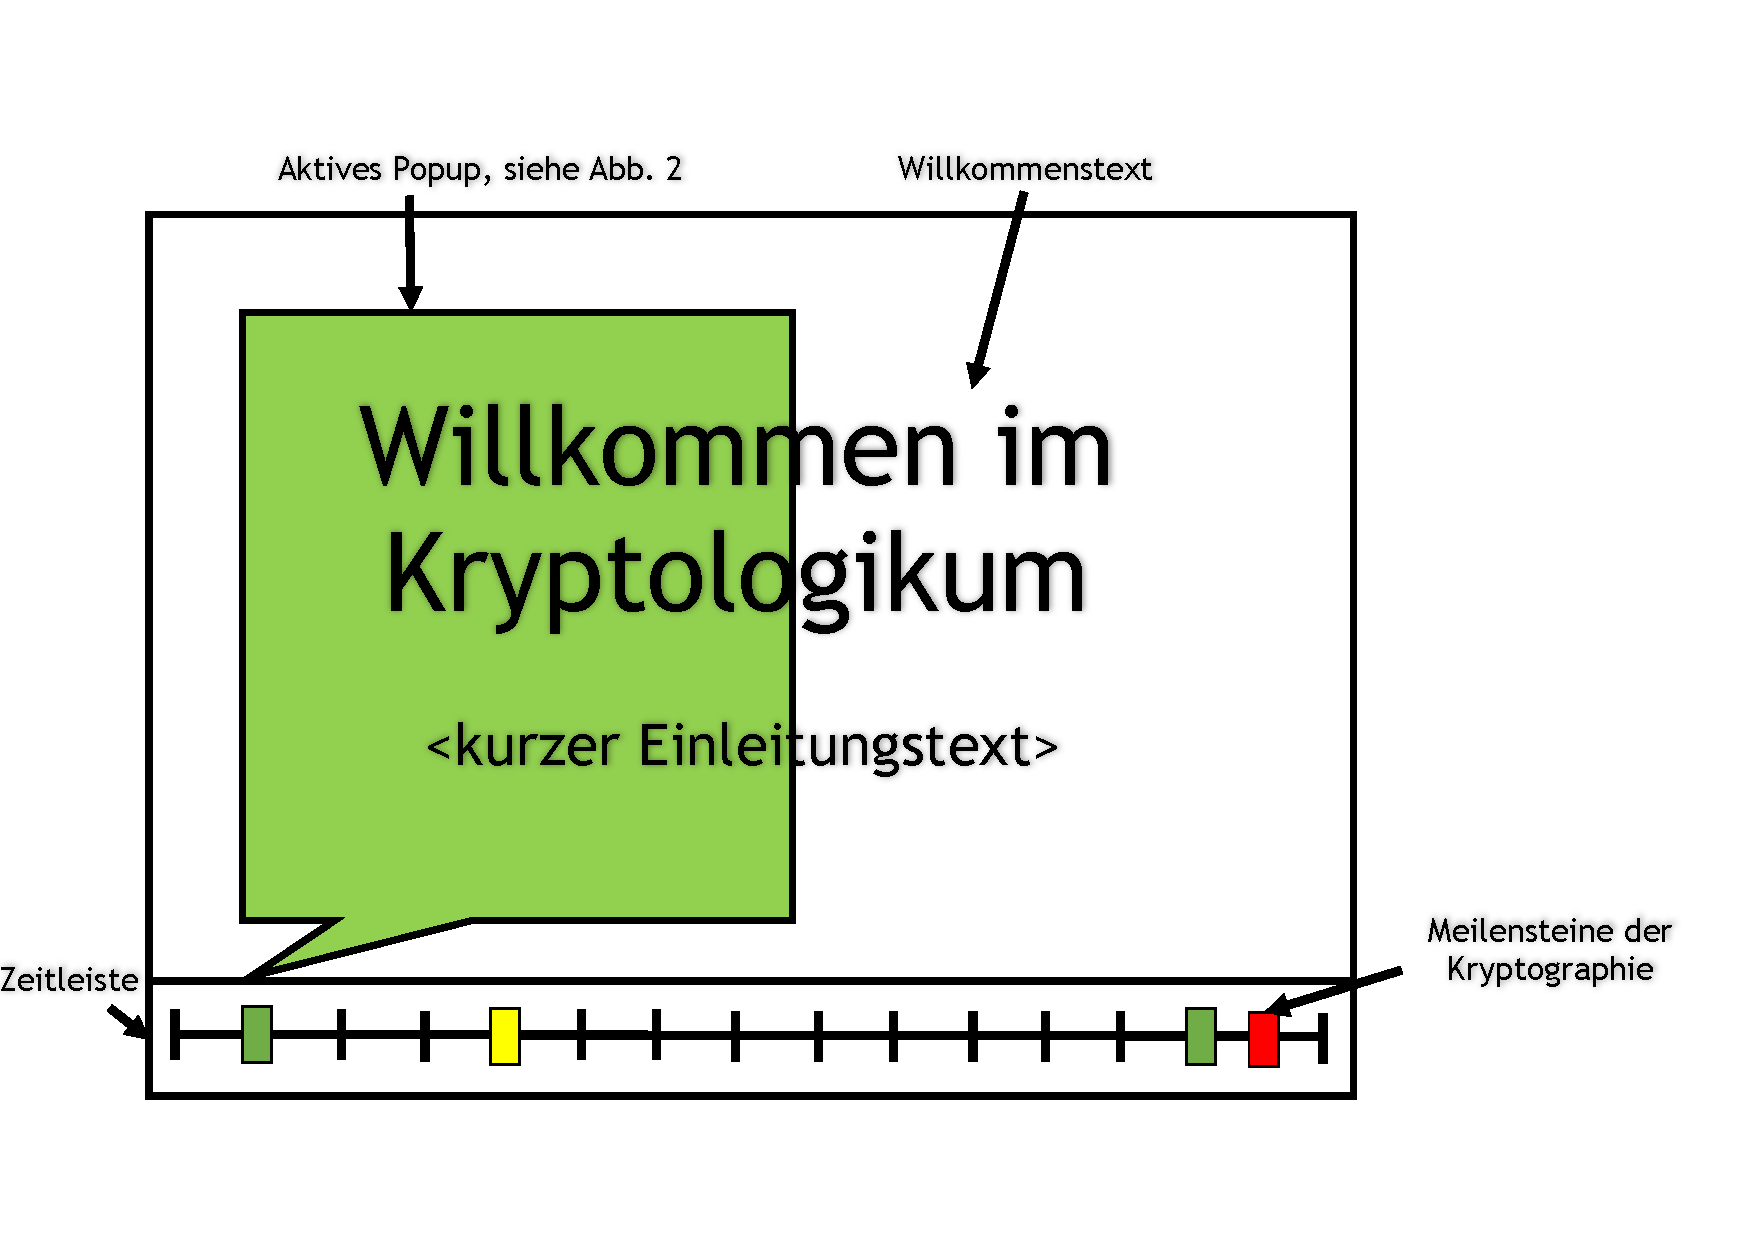
\includegraphics[width=\textwidth]{resources/ui_walkthrough_start-draft}
  \caption{Willkommensbildschirm mit Zeitleiste.}
\end{figure}

Sobald ein Meilenstein ausgewählt wurde, erscheint ein Popover (Fig. 2), dass den Namen, die Schwierigkeit und den Zweck des gewählten kryptografischen Verfahrens noch einmal zusammenfasst. Weiterhin werden ein Screenshot der eigentlichen Visualisierung sowie ein Button, um diese zu starten, dargestellt.

\begin{figure}[H]
  \centering
    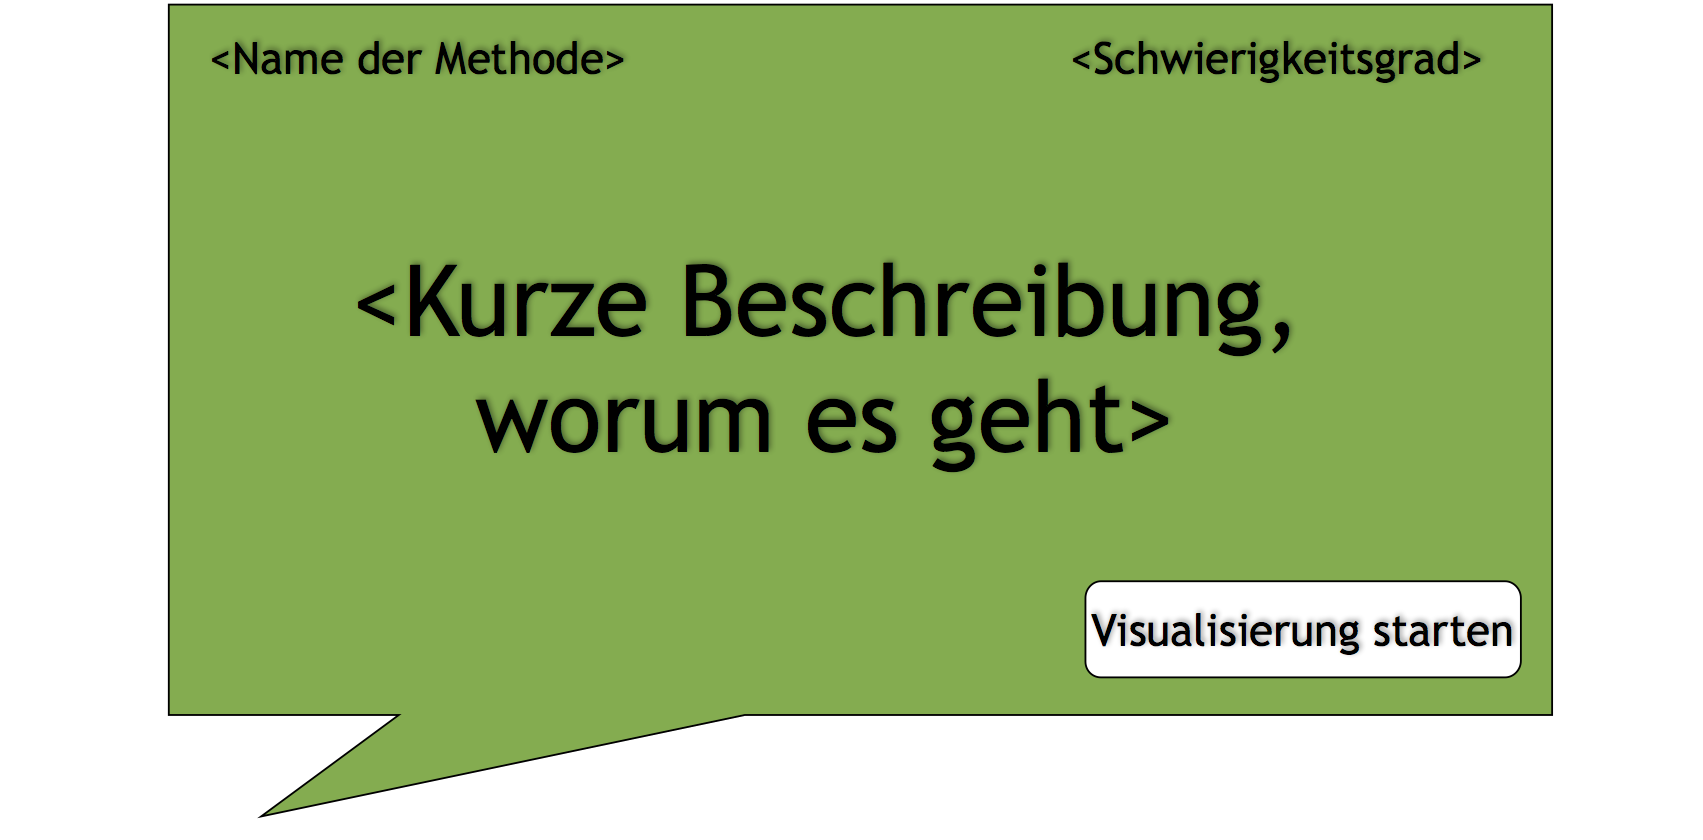
\includegraphics[width=\textwidth]{resources/ui_walkthrough_popover-draft}
  \caption{Detailansicht des Popovers in Fig. 1.}
\end{figure}

Nachdem der Benutzer eine Visualisierung startet, wird diese angezeigt (Fig. 3). Hierbei ist hervorzuheben, dass der Benutzer zu jedem Zeitpunkt die Visualisierung abbrechen kann, indem er auf den Button in der oberen linken Ecke klickt. Hilfe erhält er zu jedem Zeitpunkt im rechten oberen Eck.

\begin{figure}[H]
  \centering
    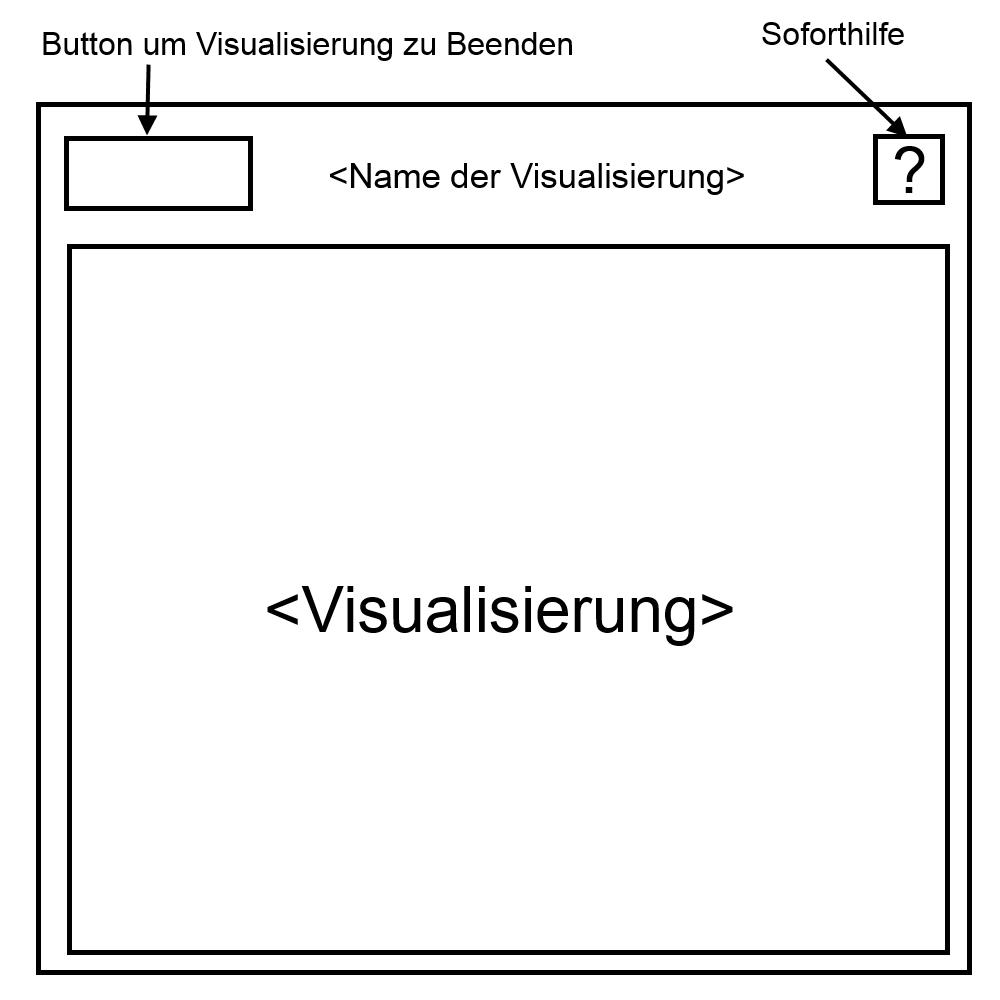
\includegraphics[width=\textwidth]{resources/ui_walkthrough_visualisation-draft}
  \caption{Darstellung einer Visualisierung.}
\end{figure}

Falls der Benutzer die Visualisierung erfolgreich beendet hat, wird (Fig. 4) angezeigt. Zunächst wird dem Benutzer zu seinem Erfolg gratuliert. Weiterhin besteht die prominente Möglichkeit, zum Willkommensbildschirm zurückzukehren. Falls das Interesse des Benutzers geweckt wurde, kann er zu (Fig. 5) wechseln.

\begin{figure}[H]
  \centering
    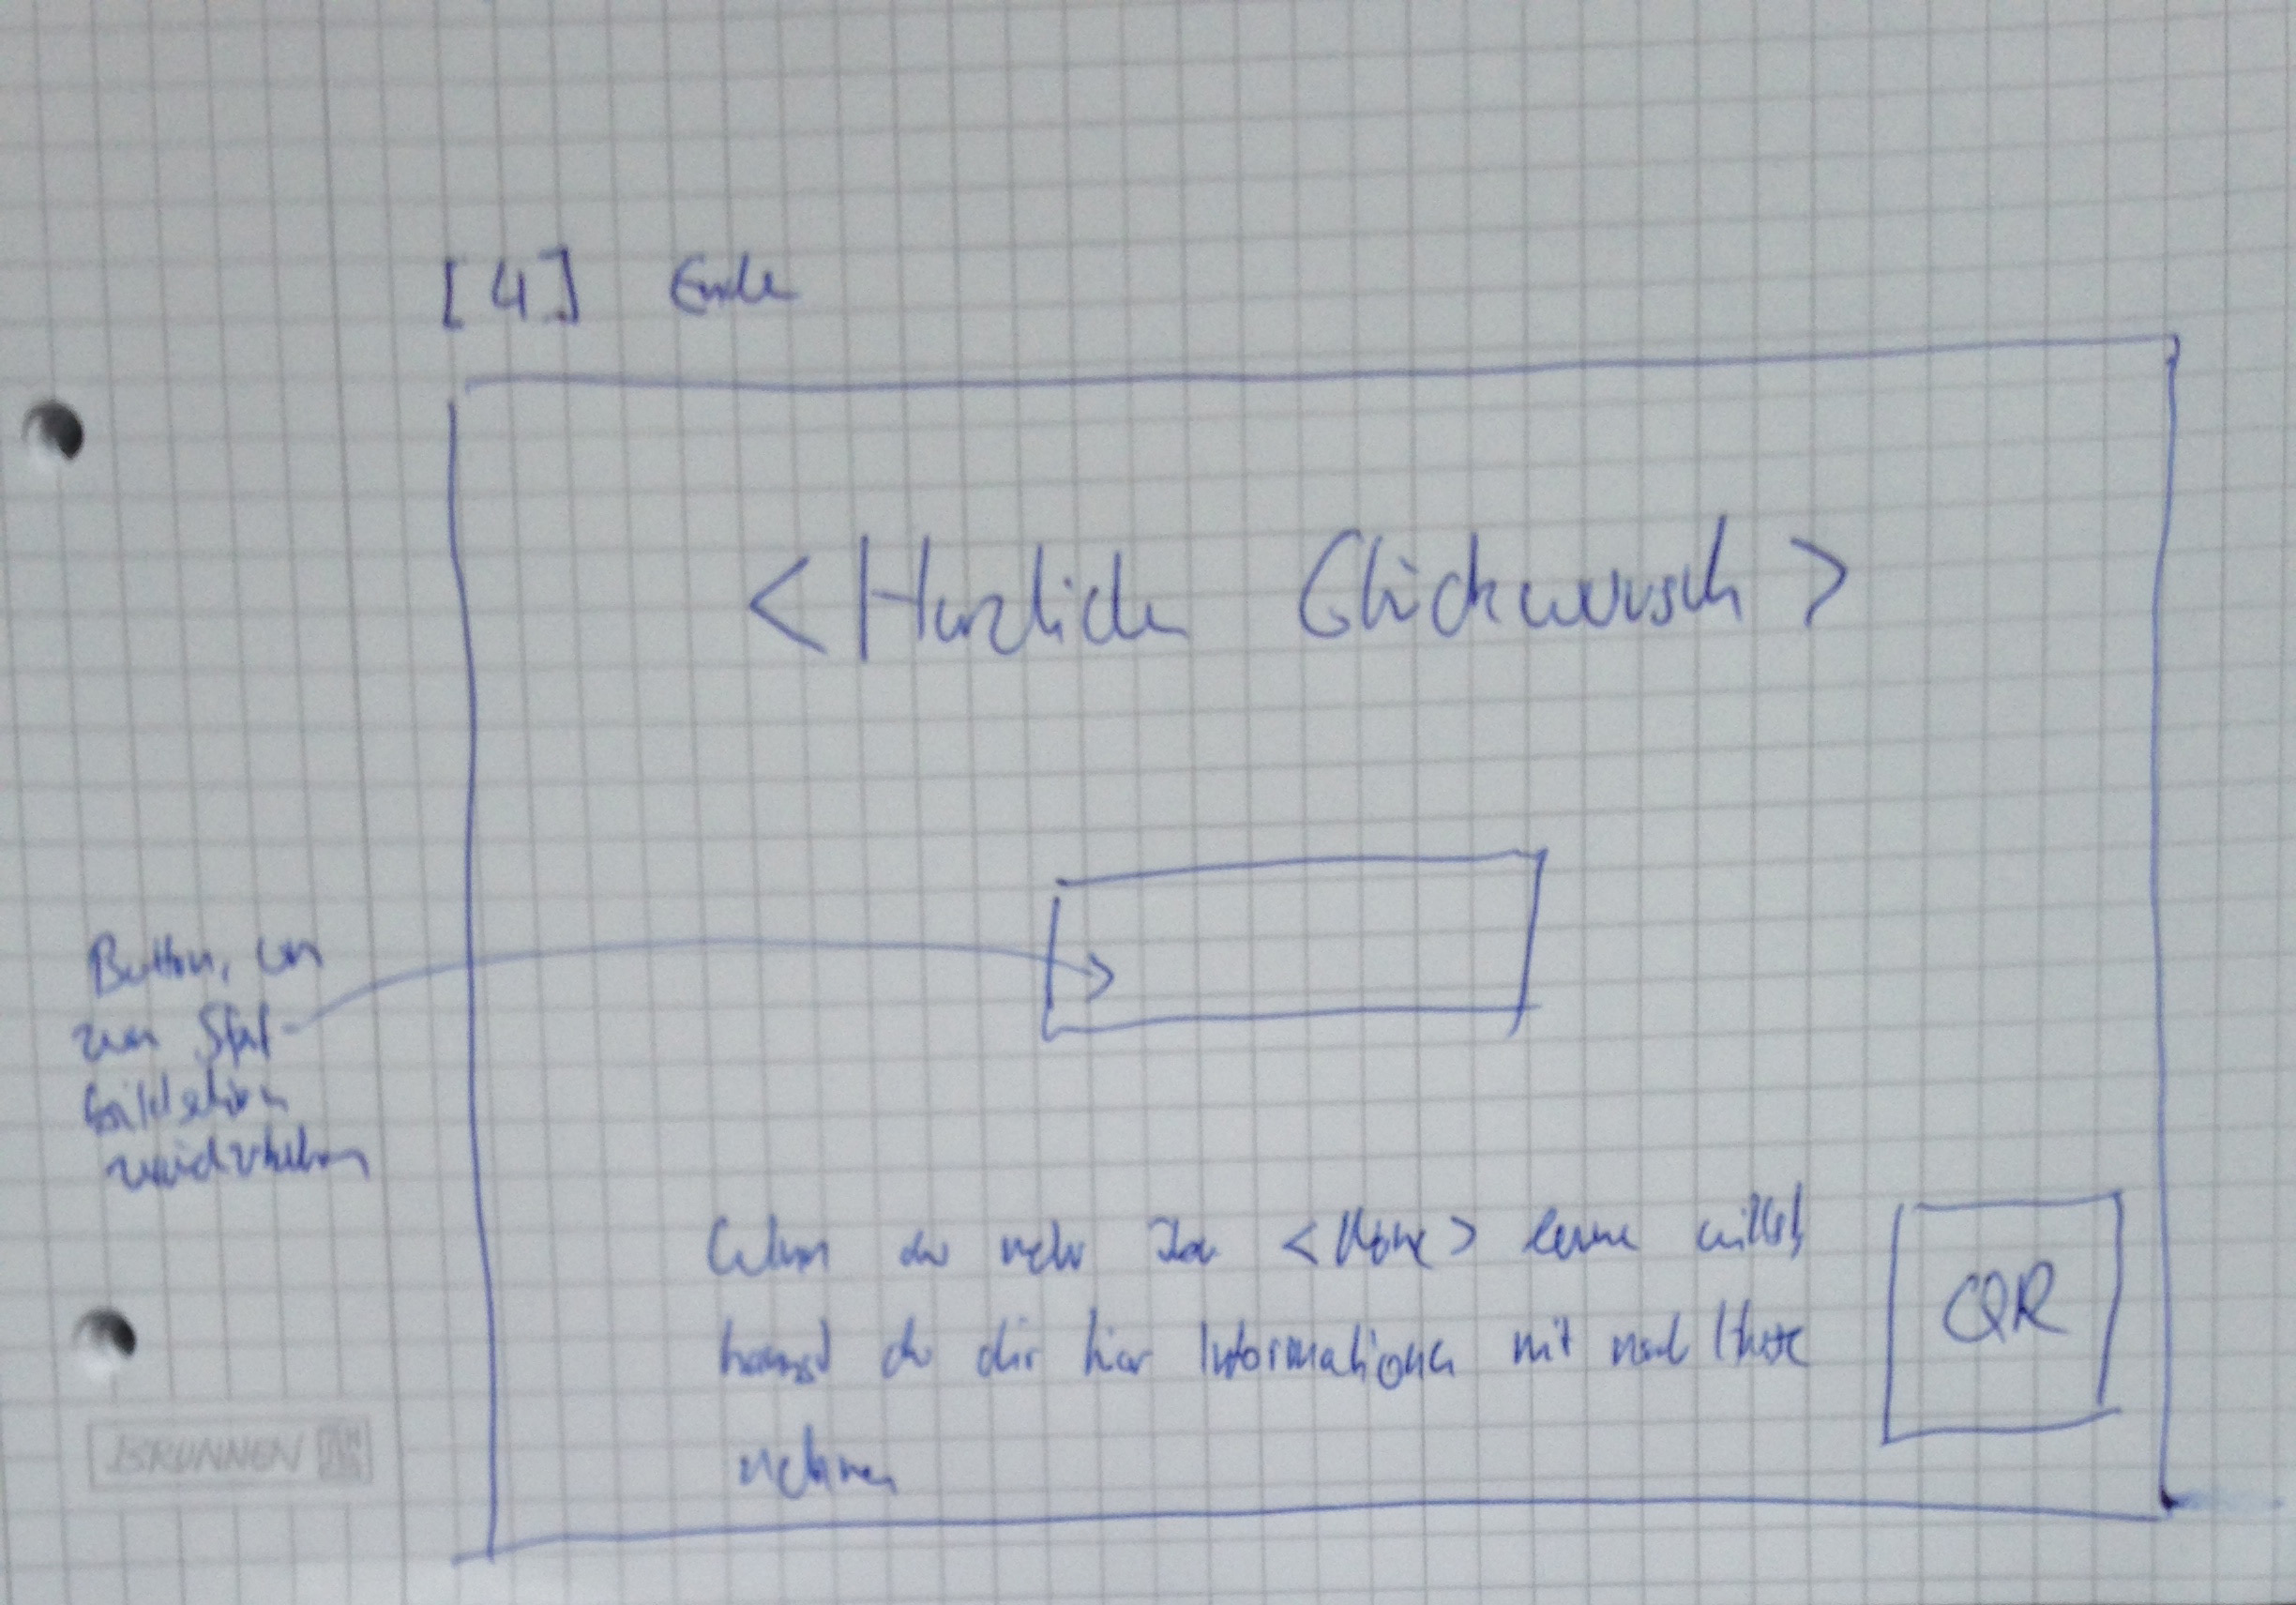
\includegraphics[width=\textwidth]{resources/ui_walkthrough_end-draft}
  \caption{Erfolgreiches Beenden einer Visualisierung.}
\end{figure}

Hier bekommt der Benutzer weiterführendes Material über sein zuvor gewähltes Thema. Außer dem Text mit den Quellen, kann auch ein QR-Code angezeigt werden, welcher vom Nutzer gescannt werden kann. Auch hier bietet sich die Möglichkeit wieder zum Hauptmenü zurückzukehren.

\begin{figure}[H]
  \centering
    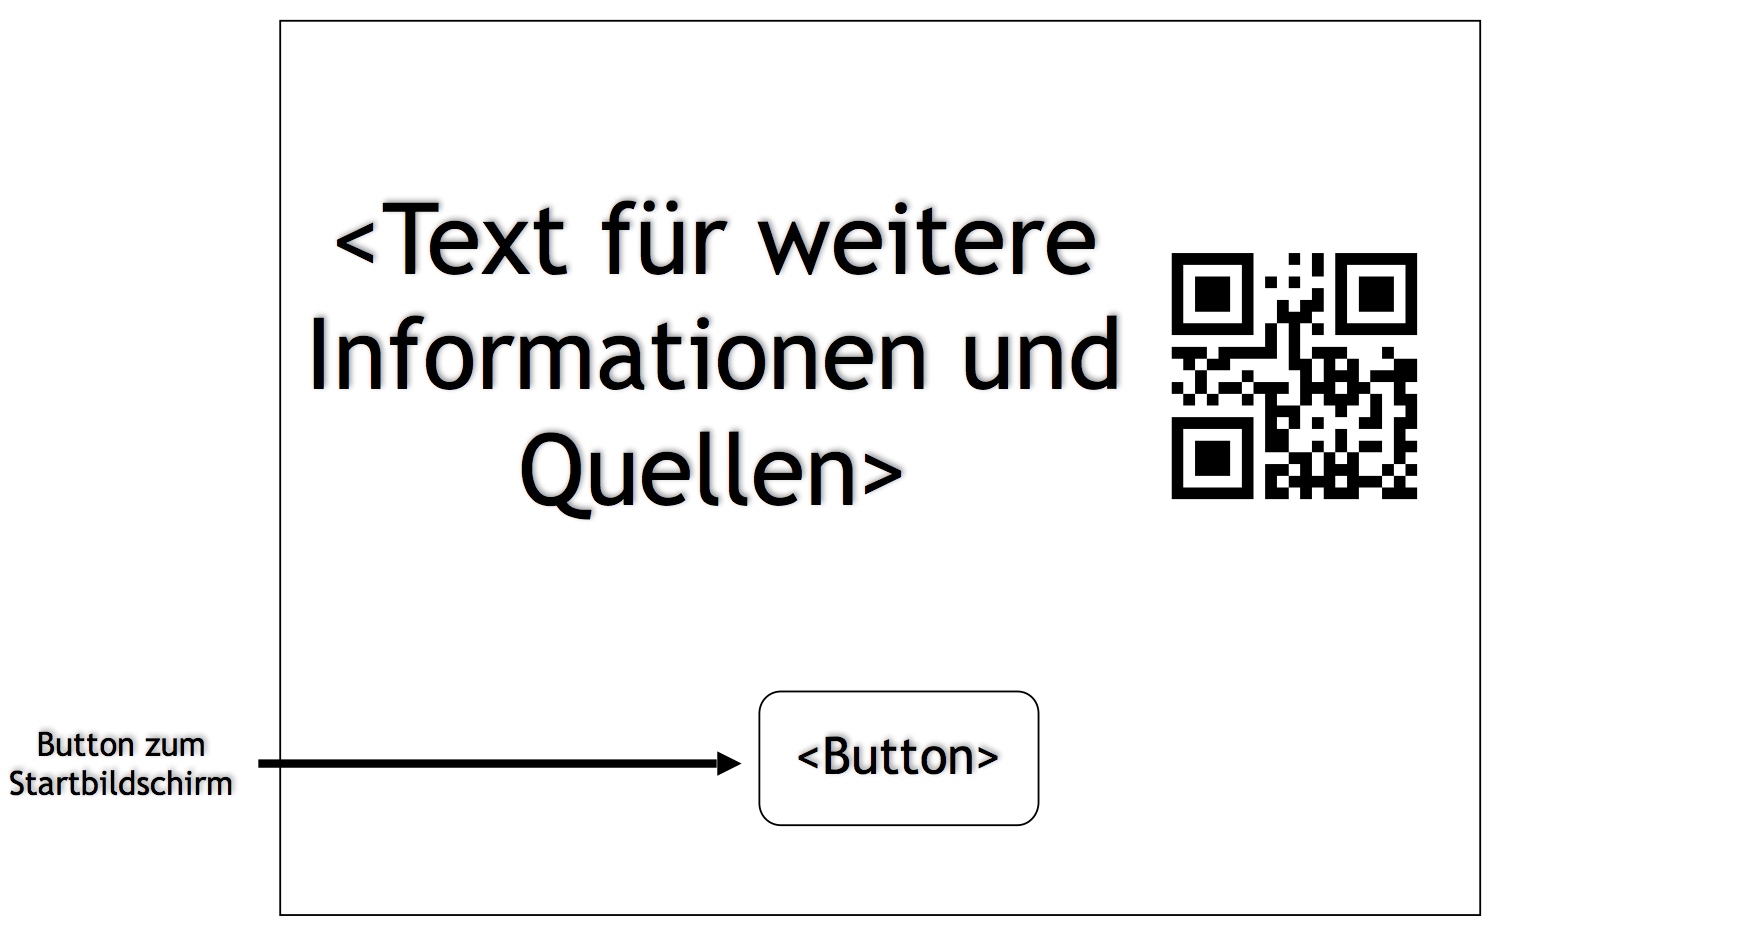
\includegraphics[width=\textwidth]{resources/ui_walkthrough_other}
  \caption{Weiterführende Informationen.}
\end{figure}


\section{Systemmodelle}

\subsection{Systemübersicht}
Das System verwendet das bekannte MVC-Entwurfsmuster. Weiterhin ist geplant, das System in zwei Schichten zu unterteilen. Von unten nach oben enthält Schicht 1 wiederverendbare und in sich abgeschlossene Bibliotheken. Zum einen handelt es sich hierbei um Code von Dritten (z.B. um QR-Codes zu generieren). Weiterhin ist eine Sammlung wiederverwendbarer Klassen (nachfolgen {\it GraphicsLib} genannt) geplant. {\it GraphicsLib} wird vor allem aus UI-Elemente bestehen, die für die Implementierung aller Visualisierungen wertvoll sind.

\begin{figure}[h!]
  \centering
    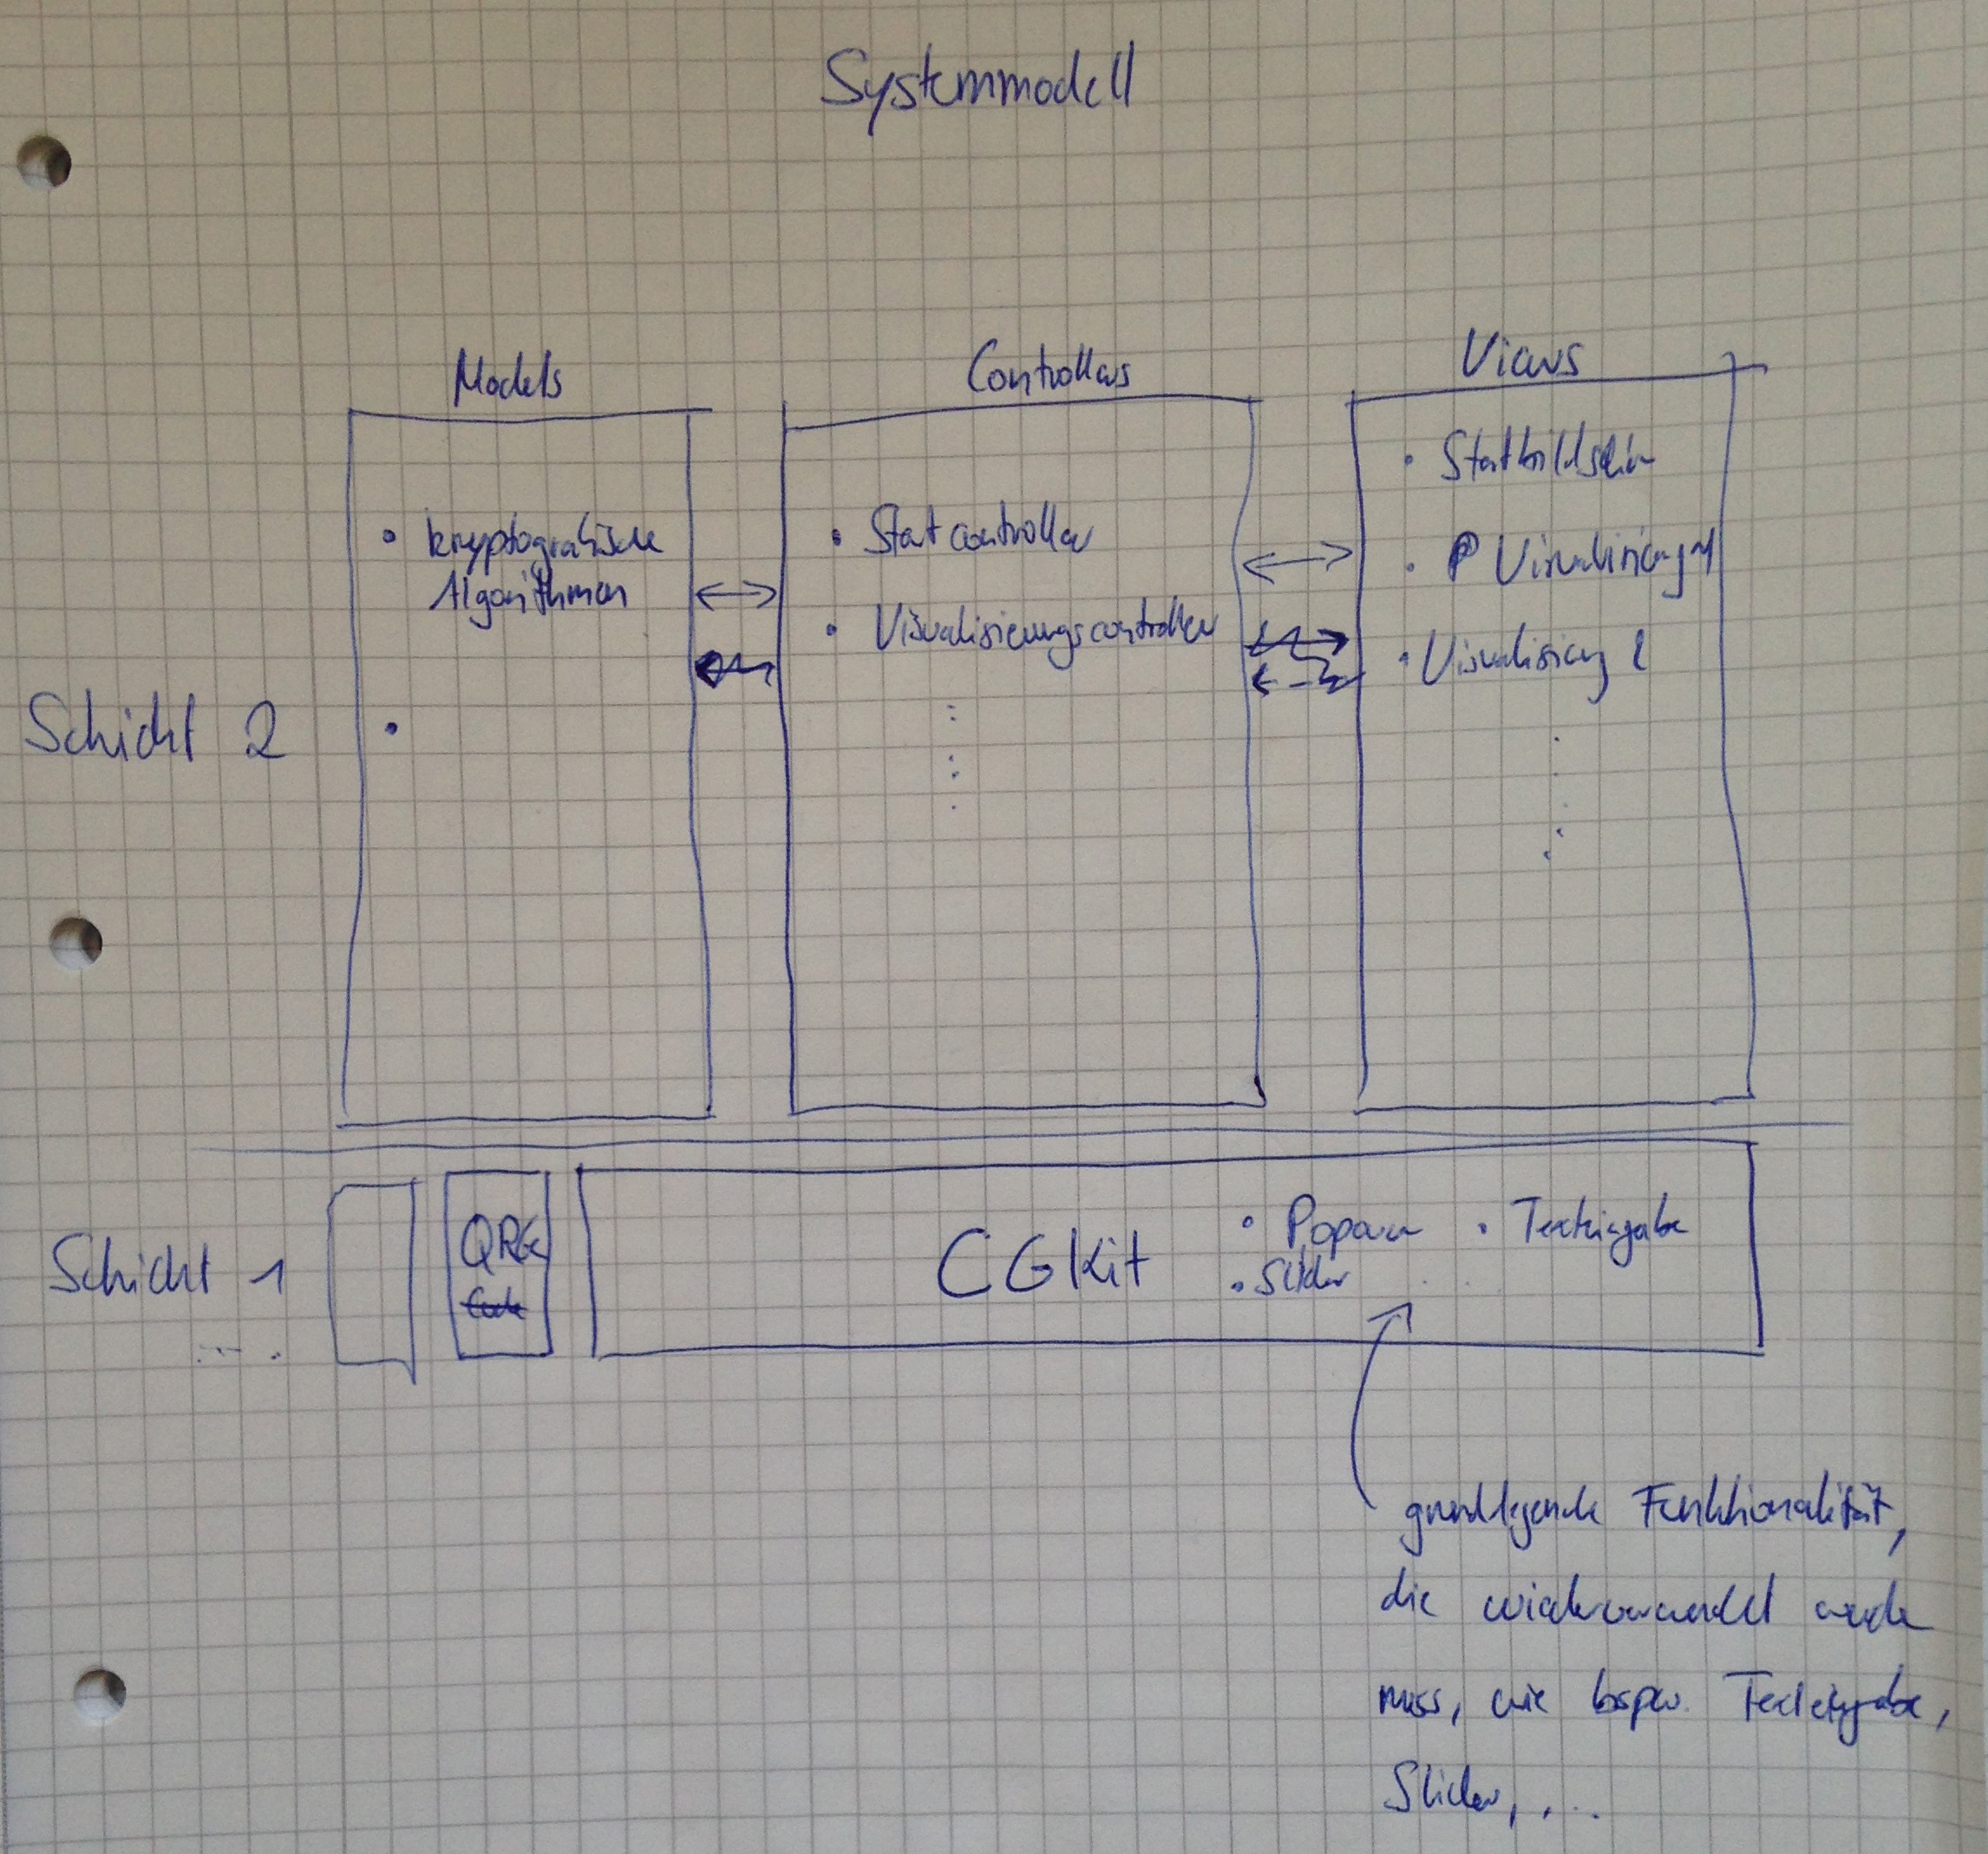
\includegraphics[width=\textwidth]{resources/systemmodel-draft}
  \caption{Schematische Darstellung des beschriebenen Systems.}
\end{figure}

\section{Beispielszenarien}
\begin{itemize}
    \item Das Beispiel läuft schrittweise ab. Problem wird dargestellt: A möchte B eine Nachricht schicken, die nicht von einer anderen Person als B gelesen werden soll. C versucht die Nachricht zu bekommen. Dabei können A und B nur über ein unsicheres Medium kommunizieren (Analogie z.B. Schlüssel per Post verschicken), das von C abgehört wird.
\item A und B generieren ihre Schlüsselpaare. Der genaue Schlüssel ist nicht relevant.
\item A fragt B nach seinem public key, den B auch bereitwillig mitteilt. C hört den public key von B.
\item A verschlüsselt die Nachricht mit dem public key von B und verschickt die Nachricht an B. C hört die verschlüsselte Nachricht ab.
\item B entschlüsselt die Nachricht von A mit seinem private key und kann die Nachricht lesen
\item C versucht mit der Nachricht irgendetwas anzufangen und versucht sie mit dem abgehörten public key von B zu entschlüsseln. Das scheitert natürlich.

Beispiel einer Visualisierung anhand des Caesar-Algos:

\item Es wird erklärt, dass vermutlich Caesar dieses Verfahren verwendet hat um geheime Nachrichten zu verschlüsseln
\item Erklärung des Prinzips an einem Beispielsatz. Es werden schrittweise alle gleichen Buchstaben markiert und in ihr Äquivalent umgewandelt (z.B. "Hallo, wie geht's?" -> zuerst alle H zu K, dann alle a zu d, dann alle l zu o). Hier gibt es die Möglichkeit, schrittweise durchzugehen und noch mal zurück zu gehen. Außerdem kann man wenn man das Prinzip verstanden hat ans Ende springen.
\item Als nächstes muss die Person ein Wort selbst verschlüsseln mit Vorschrift (z.B. a -> b).
\item Am Ende wird mithilfe eines Diagrammes und der Kenntnis, das E der häufigste Buchstabe im Deutschen ist gezeigt, dass man diese Verschlüsselung leicht umgehen kann
\end{itemize}

\textbf{Szenario 1}:
Bob ist interessiert in Kryptographie und besucht zu diesem Anlass das \gls{Kryptologikum}, um mehr Informationen diesbezüglich zu erhalten. Er nähert sich dem \gls{Cryptographics}, wo ein Bildschirmschoner verschiedene kryptographische Verfahren Teaser-ähnlich visualisiert. Eine Berührung des Bildschirmes zeigt die Willkommensoberfläche von \gls{Cryptographics}: Ein Zeitstrahl, auf dem chronologisch angeordnet verschiedene kryptographische Verfahren, ihrem Erfindungsjahr zugeordnet, genannt werden und farblich durch ihre Komplexität von grün (leicht) bis rot (schwer) gekennzeichnet sind. Bob wählt durch eine Berührung die Cäsar-Chiffre aus, sie befindet sich nämlich ganz am Anfang des Zeitstrahls. Daraufhin erscheint eine kurze Einleitung als Popup, im Hintergrund baut sich die Oberfläche auf und der Zeitstrahl gleitet verkleinert als Gesamtübersicht an den unteren Bildschirmrand. Nach dem Durchlesen der Einleitung schließt Bob das Popup, und er sieht eine Demonstration der Cäsar-Chiffre als Schritt-für-
Schritt-Beispiel auf 
einer speziell für das Verfahren ausgelegten Oberfläche. Auf genau dieser Oberfläche kann Bob nach dem Beispiel sein neu erlerntes Wissen über das Verfahren anwenden, um Texte zu verschlüsseln, und durch einen gegebenen Schlüssel zu entschlüsseln. Nachdem er das Verfahren nun verinnerlicht hat, kann Bob das nächste Verfahren auswählen, entweder durch Drücken der “Weiter”-Taste, oder indem er ein Verfahren direkt am Zeitstrahl auswählt. Da er die weiteren Verfahren auch noch sehen möchte, arbeitet er sich am Zeitstrahl entlang durch das Programm, wobei er dann schließlich auf das Diffie-Hellman-Verfahren trifft, über welches er noch mehr Informationen erhalten möchte. Er berührt einen dafür vorgesehenen Button, welcher ein Popup mit einem QR-Code öffnet, dass letztendlich zu den ausführlichen Quellen weiterleitet. Alternativ ist dort auch eine gekürzte URL zu finden die man schnell abschreiben kann (Bsp.: http://goo.gl/abcd12).\\

\textbf{Szenario 2}:
Die ungeduldige Alice wurde von ihrer Freundin überredet, an der Ausstellung teilzunehmen. Sie sieht das \gls{Cryptographics} und versucht, es durch wiederholte zufällige Eingaben zum Absturz zu bringen. Das Programm zeigt sich jedoch schnell als zu robust, um einem solchen Angriff zu erliegen. Schließlich wählt sie das komplizierteste kryptographische Verfahren aus, um Besuchern nach ihr den Einstieg zu erschweren. Nachdem sie gegangen ist, muss sie jedoch enttäuscht feststellen, dass der nächste Besucher keine weitere Schwierigkeiten hatte, das Programm mit dem dafür vorgesehenen Button in den Grundzustand zurückzuversetzen.\\

\textbf{Szenario 3}:
Nachdem Bob nun längere Zeit an \gls{Cryptographics} verbracht hat, blickt er erschreckt auf die Uhr um festzustellen, dass es schon viel zu spät geworden ist. Er bricht auf, und lässt das Programm genau so zurück, wie er es gerade eben noch benutzt hat. Nach seiner letzten Interaktion erscheint nach x Sekunden eine Meldung, die Bob darauf hingewiesen hätte, dass sich das Programm bald zurücksetzt, sollte in den nächsten y Sekunden keine Eingabe mehr erfolgen. Da er jedoch schon an der Bushaltestelle steht, aktiviert \gls{Cryptographics} nun den Bildschirmschoner, den Bob zuvor auch schon vorgefunden hatte, und setzt im Hintergrund das Programm wieder auf den Ursprungszustand zurück.\\

\textbf{Szenario 4}:
Die Ausstellung ist für diesen Tag nun zu Ende, und die Krypto-logikum-Administratorin Claudia schließt gerade noch die Tür hinter Bob ab, um sich jetzt den strombetriebenen Exponaten zu widmen. Als sie am \gls{Cryptographics} ankommt, versucht sie zunächst, irgendwie zum Betriebssystem zurückzukehren, um den PC sicher herunterfahren zu können. Nach kurzer Zeit stellt sie fest, dass das ohne eine zusätzlich eingesteckte Hardware-Tastatur auf keinen Fall möglich ist. Sie holt also eine USB-Tastatur, steckt sie ein, kehrt über den Windows-Taskmanager zum Betriebssystem zurück, fährt den PC herunter und macht die Lichter aus.\\

\begin{figure}[h!]
  \centering
    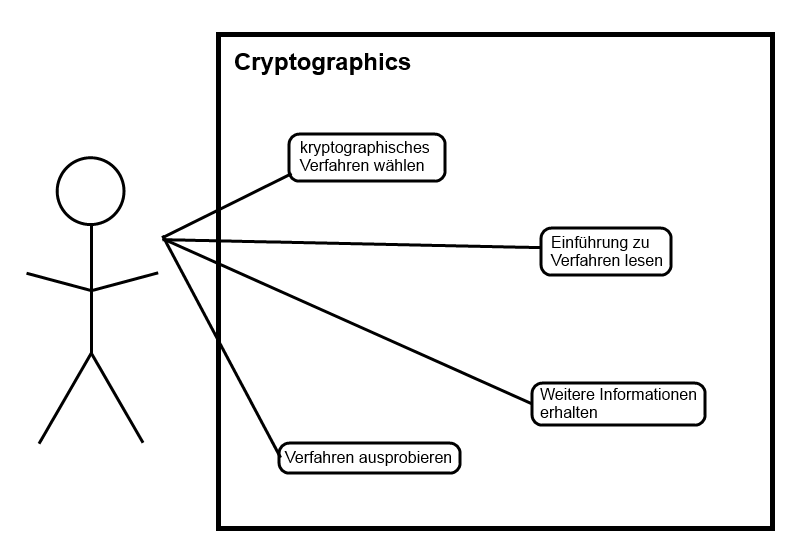
\includegraphics[width=\textwidth]{resources/usecase1}
  \caption{Anwendungsfalldiagramm zu beschriebenen Szenarien.}
\end{figure}

\section{Globale Testfälle}
- automatisiertes Testen mithilfe von JUnit vor allem der Krypto-Algorithmen
- ggf. automatisiertes Testen der UI mithilfe von Szenarien und geeignetem Framework
Stresstest mit möglichst zufälligen und willkürlichen Eingaben (wie es Kinder eben tun)
Usability Tests mit passenden Testpersonen\\
Es ist sehr ratsam, dass die globalen Testfälle mit /Txy/ sich auf die Funktionalität /Fxy/ beziehen. So ist eine gewisse Konsistenz, Überdeckungsgrad und Übersichtlichkeit gewährleistet. Folgt demnächst, wenn die Funktionalen Anforderungen fertig sind!

\section{Qualitätsbestimmung}

\section{Anhang}

\subsection{Zeichnungen, Skizzen, etc.}

-Hier können wir ggf. die Zeichnungen und Skizzen anhängen (analog wie bei Handyverträge)...-

%Glossar ausgeben
\glsaddall
\printglossary[numberedsection, style=altlist]

\end{document}
